\section{Implementierung}\label{sec:implementierung}
%TOTO LEFTOVER: 
%QUIZ
%HTTPS
%WLAN
Das folgende Kapitel wird Einblicke in die Entwicklung der Software im Rahmen des Projekts geben. 
Dabei wird iterativ chronologisch die Vorgehensweise schriftlich reflektiert und an mehreren Stellen 
zum besseren Verständnis auch ein Einblicke in den Sourcecode gegeben. Anknüpfend werden etwaige Probleme bei der Implementierung aufgezeigt sowie mögliche Lösungen diskutiert. 

\subsubsection{Implementierung der Server-Software}\label{sec:implementserver}
Aufbauend auf das Entwurf Kapitel soll die Server-Software mit NodeJS und ExpressJS als Hauptkomponente entwickelt werden. Dazu wird zunächst im folgenden Abschnitt \ref{sec:implementexpress} der HTTP Server grundlegend konfiguriert und anschließend dessen Routen im darauffolgenden Kapitel \ref{sec:anlegrouten} angelegt. 

\subsubsection{ExpressJS Setup}\label{sec:implementexpress}
Nachdem das Projekt grundlegend mit dem Befehl \texttt{npm init} initialisiert wurde,
kann ExpressJS einfach über den Node Packet Manager (nachfolgend NPM genannt) hinzugefügt werden. 
Zusätzlich wird das NPM Paket IP genutzt um die aktuelle IP-Adresse der Maschine zu automatisch ermitteln und
den ExpressJS Server auf dieser lauschen zu lassen. Dies ist mit wenigen Zeilen Code erledigt:
\begin{lstlisting}[caption=Errichtung des Webservers]
const app = express();
const server = app.listen(3000, server_ip, function () {
logger.log({ level: 'info', message: `Hello! The Server is running on ${server_ip}!`});
});
\end{lstlisting}
Der Server lauscht auf der IP Adresse des Adapters der Maschine auf dem er ausgeführt wird, zusätzlich auf Port 3000, dies sollte je nach Konfiguration auf den Standard HTTP Port 80 resp. 443 geändert werden, sollte Verschlüsselung eingerichtet sein (HTTPS).
\\
Anschließend können nun die Routen eingerichtet werden.

\subsubsection{Autarkes WLAN}\label{sec:eigeneswlan}
Um einen Stand-Alone Betrieb\footnote{Stand-Alone meint einen Betrieb unabhänging von ggf. vorhandenen Netzwerkinfrastruktur am Einsatzort} der Software zu ermöglichen, wird als Lösung der Betrieb eines unabhängigen kabellosen Netzwerkes (WLAN/Wifi) angestrebt. Folgende mögliche Lösungsszenarien wurden ausgearbeitet.
\begin{enumerate}
	\item \textbf{Einfach}: Als einfachste Lösung hat sich der Betrieb eines lokalen WLANs über ein Smartphone oder Laptop herausgestellt. Nahezu jedes Smartphone bzw. jeder Laptop lässt das generieren eines WLAN Zugangspunkt für andere Geräte zu. Der Server wird mit diesem Netzwerk verbunden, sowie alle Clients. Dies wurde getestet und ein Betrieb war möglich. Da hierbei aber auch die Internetverbindung des Zugangspunktes freigegeben wird, was ggf. unerwünscht sein kann, würde es sich anbieten eine spezielle 'Companion App' zu entwickeln und für Android / iOS basierte Smartphones zu entwickeln. Diese könnte automatisch einen WLAN-Hotspot erstellen und den Netzwerkverkehr eventuell limitieren. Gleiches gilt analog für windows- oder unixbasierte Computer, ist aber problematischer, siehe dazu nächsten Listenpunkt.
	\item \textbf{Speziell}: Um auf einem Computer vollautomatisch einen WLAN Hotspot zu genieren, bedarf es Administrator Privilegien sowie genauere Kenntnisse über den verwendeten Netzwerkadapter. NodeJS selbst bietet nur eingeschränkt Möglichkeiten an, diese Aufgabe autark zu übernehmen, könnte aber ggf. eventuelle Shell-Skripte triggern. Unter Microsoft Windows 7+ gibt es mit den NPM Paket \texttt{node-hotspot} auch die Möglichkeit, dies direkt mit NodeJS zu erledigen. Diese Paket wird in die zu entwickelnde Software integriert und soll anschließend unter einer Microsoft Windows Umgebung das generieren eines WLAN Hotspots / Zugangspunktes ermöglichen. Zur Verwendung werden entsprechende Steuerungsoptionen in Einstellungsbereich im Lehrkraft Backend integriert. Die interne Steuerung erfolgt über Routen (siehe auch Abschnitt \ref{sec:anlegrouten}).
	
Wird die Applikation in einer vorhandenen Netzwerkinfrastruktur betrieben, ist ein Betrieb in jedem Falle gewährleistet. Ein mobiler WLAN-Router könnte ebenfalls genutzt werden, sollte keine ausreichende Infrastruktur vorhanden sein. Dieser müsste einmalig konfiguriert werden und ist anschließend in der Lage die Serverapplikation für Clients ansprechbar zu machen. Ein solches Gerät gibt es bereits ab ca. 10 Euro zu erwerben.
\end{enumerate} 

\subsubsection{Verschlüsselung}\label{sec:encrypted}
Um eine verschlüsselte Kommunikation zwischen Server und Clients zu gewährleisten, ist der Datenaustausch über das HTTPS Protokoll vorzuziehen. Um HTTPS allerdings sinnvoll nutzen zu können, ist ein Zertifikat von einer Zertifizierungsstelle (CA) notwendig, was meist mit Kosten verbunden ist. Allerdings bietet der Anbieter \textbf{Let's Encrypt}\cite{LetsEncrypt.org} kostenlose Zertifikate an, welche sich problemlos bei vorhandenem SSH-Zugang installieren lassen. Für den Intranet Betrieb können relativ einfach eigens ausgestellte Zertifikate genutzt werden, welche mit Shell-Programmen wie \textbf{openssl} generierbar sind\cite{Copes2018}. Allerdings warnen moderne Webbrowser den Nutzenden recht auffällig, dass die genutzte Verbindung dennoch nicht sicher ist, da dem Zertifikat nicht vertraut werden kann. Der HTTPS Betrieb wurde erfolgreich getestet. Die Implementierung ist nicht aufwendig allerdings, birgt aber den o.g. Nachteil. Da das Intranet ein an sich abgeschlossenes Netzwerk ist, scheint der verschlüsselte Betrieb in diesem zunächst nicht wichtig, kann aber jederzeit realisiert werden und ist bei Betrieb im Internet als obligatorisch zu betrachten. 

\subsubsection{Anlegen der Routen}\label{sec:anlegrouten}

Grundlegend soll es folgende Routen auf dem Server geben:
\begin{itemize}
	\item \textbf{'/'}: Die Haupt Route, sie wird angesteuert, wenn der Server einfach unter seiner IP (oder eingerichteter Domain) kontaktiert wird. Hier wird anschließend die Rolle des Nutzers (Lehrender oder Schülerin/Schüler) abgefragt  und dementsprechend weitergeleitet.
	\item \textbf{'/teacher'}: Diese Route verweist auf den Lehrerbereich der Anwendung, man kann sie auch als Backendbereich bezeichnen. Alle hinter dieser Route liegende Routen bedürfen einer Authentifizierung seitens des Nutzenden.
	\item \textbf{'/client'}: Diese Route verweist grundlegend auf den Student Client. Aber auch der Presenter Client wird über diese Weiche aufgerufen. 
\end{itemize}
Neben diesen drei Hauptrouten existieren noch weitere spezial Routen für das Error-Handling (z.B. 404 - Seite nicht gefunden) sowie besondere für die WebSocket Kommunikation, welche aber im Hintergrund genutzt werden und im Abschnitt \ref{REF UNKNOWN YET!} beleuchtet werden.\\ 
Das Anlege der Routen ist mit folgendem Codeausschnitt durchgeführt:
\begin{lstlisting}[caption=Anlegen der Routen]
app.use('/teacher', teacherRoutes);
app.use('/client', clientRoutes);
app.use('/', mainRoutes);
\end{lstlisting}
\footnotesize{Die Route Module werden im Hauptmodul (app.js) referenziert und deren Zuständigkeit festgelegt.}
\normalsize
Zu beachten gilt: Die weiterführend Routen werden in Dateien ausgelagert, um die Übersicht des Quelltextes zu wahren. Ebenso sind auch diese Routen sog. Middleware-Funktionen. Dies wird im nächsten Abschnitt genauer beleuchtet. Daher ist auch die Reihenfolge wichtig, würde die \texttt{'/'} Route als erstes angelegt werden, so würde diese alle folgenden, spezifischeren 'abfangen'.  


\subsubsection{Reflexion des MVC Schemas}\label{sec:mvc}
Da der Server nach dem Model-View-Controller Muster grundlegend arbeiten soll, gilt es dieses zu implementieren. Die folgende Tabelle soll ein Überblick über die anfallende Struktur geben:

\begin{table}[h!]
	\caption{MVC Struktur der Implementierung}
	\label{tab:mvcschema}
	\begin{tabular}{|l|l|l|l|}
		\hline
		\multicolumn{1}{|c|}{\textbf{Betrifft}}                         & \multicolumn{1}{c|}{\textbf{Model}} & \multicolumn{1}{c|}{\textbf{View(s)}}                                                                         & \multicolumn{1}{c|}{\textbf{Controller}}                                            \\ \hline
		Lehrende                                                        & user.js                             & \begin{tabular}[c]{@{}l@{}}teacher/new.pug\\ teacher/signup.pug\\ teacher/user-edit.pug\end{tabular}          & teacher.js                                                                          \\ \hline
		\begin{tabular}[c]{@{}l@{}}Schülerinnen/\\ Schüler\end{tabular} & student.js                          & student.pug                                                                                                   & client.js                                                                           \\ \hline
		Lehreinheiten                                                   & eduSession.js                       & \begin{tabular}[c]{@{}l@{}}edusessions/*/*.pug\\ edusessions/index.pug\\ edusessions/running.pug\end{tabular} & \begin{tabular}[c]{@{}l@{}}session.js\\ quizzing.js\\ brainstorming.js\end{tabular} \\ \hline
	\end{tabular}
\footnotesize {
	Zum Zwecke der Übersicht wurden einige interne Controller-Dateien nicht gelistet, wie z.B. der Error-Controller, welcher zwar eine View besitzt, jedoch kein Model. 
}
\end{table}
\newpage
Folglich müssen die entsprechenden Controller-Funktionen an Routen gebunden werden. Dabei wurde sich teils am RESTful Design orientiert, die Umsetzung erhebt jedoch kein Anspruch vollkommen 'RESTful' zu sein. Zunächst müssen entsprechende Unterrouten zu den aus Abschnitt \ref{sec:anlegrouten} bereits angelegten hinzugefügt werden. Zwecks der Übersicht wird hierzu ein Routes Ordner angelegt, welche die entsprechenden Router enthalten soll. 
Folgende Router werden angelegt: \\ \\
\textbf{routes/client.js}: Legt alle Student Client und Presenter Client relevanten Routen fest.\\
\textbf{routes/teacher.js}: Alle für das Backend resp. Lehrerbereich relevanten Routes werden hier angelegt.\\
Es folgt ein Codebeispiel aus der Datei routes/client.js. 
\begin{lstlisting}[caption=Unterrouten und Controlleranbindung]
// 3rd Party Imports
const express = require('express');
const router = express.Router();
// App Imports
const clientController = require('../controllers/client');
const isAuth = require('../middleware/is-auth');
// Presenter & Student Clients
router.get('/presenter/:sessionId', isAuth, clientController.getPresenter);
router.get('/student', clientController.getStudent);
router.get('/', clientController.getStudent);
module.exports = router;
\end{lstlisting}
Zur Verdeutlichung wird anknüpfend die in Zeile 10 des vorangegangen Listings Funktion \texttt{getStudent} des Controllers gezeigt:
\begin{lstlisting}[caption=GET Funktion des Student Controllers]
// GET => /client/student
exports.getStudent = (req, res, next) => {

return res.render('client/student',
	{
		docTitle: 'Student | Node ICT',
		ipAdd: ip.address(),
	});
};
\end{lstlisting}
 
 \subsubsection{Einrichtung der Datenbank}
 Die SQL Datenbank 'SQLite'  und der Object-Relationship-Mapper 'Sequelize' können einfach über den NPM dem Projekt hinzugefügt werden.  
 Nach diesem Schritt kann die Anbindung und Einpflegung folgen. Hierzu wird ein Datenbank Utility Modul angelegt, dieses soll die grundlegende Konfiguration der Datenbank enthalten und ausführen. All dies kann direkt über Sequelize erfolgen, welches im Hintergrund die notwendigen Schritte vornimmt. Es muss der Dialekt 'sqlite' angegeben werden und der Pfad unter welchem die Datenbank als Datei gespeichert werden soll. \\ 
 Gemäß dem logischen Aufbau einer SQL Datenbank folgt nun das Konfigurieren und Anlegen der Tabellen und deren Beziehung untereinander. Dieser Arbeitsschritt erfolgt relativ intuitiv. Im folgenden Code-Beispiel wird die Tabelle bzw. Sequelize Model 'student' im Modul tables konfiguriert.
 
 \begin{lstlisting}[caption=Anlegen einer Tabelle und deren Beziehungen]
exports.student = (sequelize, Sequelize) => {
	return sequelize.define('student', {
		id: {
			type: Sequelize.INTEGER,
			autoIncrement: true,
			allowNull: false,
			primaryKey: true
		},
		name: {
			type: Sequelize.STRING,
			allowNull: false
		},
	})
};
 \end{lstlisting}
 Im Datenbank Utility Modul wird nun die Konfiguration geladen und anschließend dessen Beziehung zu anderen Entitäten eingestellt. Durch Sequelize kann hier ein relativ humanes Sprachbild verwendet werden. Das folgende Beispiel zeigt die Beziehungen zwischen EduSession und Student an:
 \begin{lstlisting}[caption=Konfiguration von Entitätsbeziehungen]
 EduSession.hasMany(Student, { onDelete: 'cascade' });
 Student.belongsTo(EduSession);
 \end{lstlisting}
 Nach dem selben Schema werden nun für alle Modelle entsprechende Tabelle angelegt und deren Beziehungen untereinander festgelegt. 
 \paragraph{Datenbank Interaktion}
 Um Datenbank Anfragen (Queries) zu stellen, bietet Sequelize viele Optionen an. Diese müssen nicht in SQL geschrieben werden, sondern sind normale JavaScript Funktionen. Jedes innerhalb Sequelize definierte Model bietet diese automatisch an. Als Beispiel könnte nun über 
 \texttt{const studentToFind = Student.findByPk(1);} die Entität mit der ID 1 geladen werden. All diese bereitgestellten Funktionen sind JavaScript Promises, d.h. sie werden asynchron ausgeführt und es Bedarf entsprechendes Handeln im Fehlerfall.
 Im Erfolgsfall befindet sich in der Variabel nun das Objekt der Entität und dieses bietet wiederum Funktionen zur Interaktion an. Eine ausführliche Dokumentation findet sich auf der Webpräsenz von Sequelize. 
 Die in Tabelle \ref{tab:mvcschema} gelisteten Modelle werden gemäß der Arbeitsteilung des MVC-Schemas hauptsächlich direkt mit Sequelize arbeiten und den Controllern entsprechende Funktionen bereitstellen.
 \subsubsection{Implementierung des LehrerInnen Bereiches}\label{sec:implementlehrer}
 %hier halt sessions zum einlogge
 % Das Grundsetup wenn alles neu
 % User Anlegen / Freischalte / Sicherheit bei der Datenfreigabe 
 % Anlegen von Lehreinheiten + Brainstorming + Quizzing
 Nachdem die aus Abschnitt \ref{sec:mvc} genannten Model-Module angelegt wurden, welche direkt mit der Datenbank interagieren, müssen anschließend Controller für die verschiedenen Abschnitte des Webservers implementiert werden. Jedes Model hat dabei einen zugehörigen Controller, welcher entsprechende Funktionen für die Routen exportieren soll. Wie in Listing 3 beispielhaft zu sehen, wird die GET-Route '/student' mit der nach außen hin exportierten Funktion \texttt{getStudent} assoziiert. Um eine einheitliche Struktur zu gewährleisten, werden exportierte Funktionen eines Controller Moduls immer nach der jeweilig bedienten Request-Methode benannten (GET, POST, etc.). \\
 \paragraph{View Rendering mit PUG}
Für alle Views soll die Template Engine Pug zum Einsatz kommen (siehe auch Kapitel \ref{sec:konzept} Konzept). Dazu wird PUG für das Rendern aller nicht statischen Routen im Hauptmodul der Software registriert. PUG macht das Schreiben von HTML Dokumenten sehr komfortable und unterstützt Vererbung (Layouting). So wird zunächst für den LehrerInnen Bereich ein Main Layout angelegt, von dem später alle anderen, diesem Bereich zugehörigen, Views erben. Die Layouts können zusätzlich so genannte Blöcke enthalten, welche später dann dynamisch mit Inhalten von Views gefüllt werden, welche vom Main Layout erben. Die Controller können Daten an die Views übergeben, welche von diesen dann dargestellt werden. Dazu bietet PUG wie die meisten Template Engines Funktionen an, wie das Iterieren über Datensätze mittels Schleifen ermöglicht oder dynamisch generierte Inhalte abhängig von konditionalen Ausdrücken. Sämtliche an die Clients ausgelieferte HTML Dokumente sollen von PUG on-demand generiert werden. PUG benutzt seine eigene Templating-Language, welche sich deutlich von dem bekannten HTML unterscheidet, aber sehr intuitiv und schnell zu lernen ist. So wird die Hierarchie der HTML Elemente allein durch Einrückung bestimmt. Somit entfällt das Schließen dieser komplett. \\ 
Es werden anschließen für alle Modelle Views angelegt, damit Lehrende sich anmelden und einloggen sowie neue Benutzer anlegen und editieren können. Ebenso für das erstellen von Lehreinheiten vom Typ Brainstorming und Quiz. Dabei werden bei Dateneingabe seitens der Nutzende Formulare verwendet, welche anschließend via POST Request an den Server geschickt und dort von Controllern und ihren jeweiligen Modellen ausgewertet. Das tatsächliche Ausführen und dessen Entwicklung wird im später folgenden Abschnitt \textbf{\ref{sec:implementsessions} Implementierung der Lehreinheiten} beschrieben. 
\\ 
HIER NOCH EIN LISTING?
\paragraph{UI Design}
Aufbauend auf den Abschnitt \ref{sec:uientwurf} des Entwurf-Kapitels wird zur Designumsetzung das Frontend-CSS-Webframework \textbf{Bootstrap} genutzt. Dieses kann ebenfalls einfach über NPM dem Projekt hinzugefügt werden. Als Design-Theme soll das frei erhältliche Bootstrap Theme \texttt{Neat} von \textbf{freehtml5.co} die Grundlage bilden. Dieses wird gänzlich im Backend-Bereich des Lehrkraftzugangs genutzt, angepasste Teile anknüpfend für den Student Client und den Presenter Client, welche insbesondere noch durch eigenen CSS Code für die Nutzung auf Großbildgeräten wie Fernsehern und Projektoren optimiert wird. Es wird sichergestellt dass sich die Software angenehm auf stationären wie mobilen Endgeräten nutzen lässt. 

\begin{figure}[h!]
	\centering
	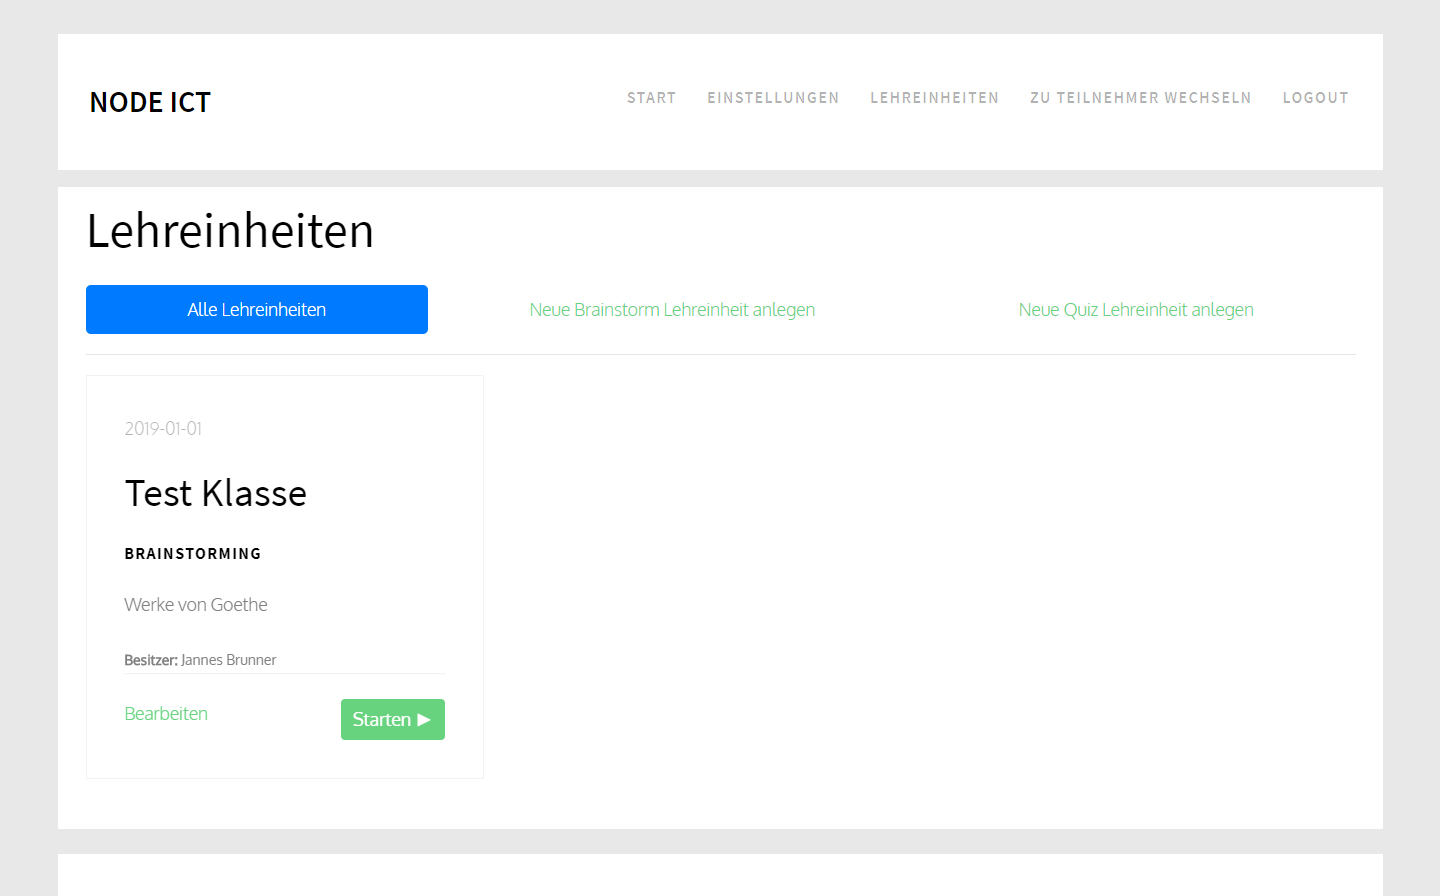
\includegraphics[width=0.9\linewidth]{bilder/screenshot_lehreinheiten}
	\caption[Screenshot UI Design Lehreinheitenbereich]{UI Design der Applikation beispielhaft illustriert durch ein Screenshot des Lehreinheiten Bereiches im Backend Zugang des Teacher Clients.}
	\label{fig:screenshot_lehreinheiten}
\end{figure}

\paragraph{Absicherung des Bereiches}
Bestimmte Bereiche der Applikation sollen nur registrierten und freigeschalteten Benutzenden zugänglich sein. Beim erstmaligen Initialisieren wird der Server mit einem Super-Administrator Account eingerichtet. Nur dieser soll neue Nutzer freischalten, andere Lehrende zu Administratoren ernennen und die Applikation auf Werkseinstellungen zurücksetzen können. Eine entsprechende Einrichtungsmaske soll beim ersten Serverstart automatisch erscheinen. Um dies technisch zu realisieren, wird das aus dem \textbf{Konzept} Kapitel genannte \texttt{express-session} NPM-Modul genutzt, welches bereits vollständig mit der von Sequelize verwalteten SQLite Datenbank einsatzbereit ist. Nach der Einrichtung im Hauptmodul wird eine eigene Middleware geschrieben, welche bei allen abgesicherten Routen als erstes aufgerufen wird und überprüft, ob die vom Client übertragene Session noch gültig ist.
\begin{lstlisting}[caption=Code der Authentifizierungs Middleware]
module.exports = (req, res, next) => {
	if(!req.session.isLoggedIn) return res.redirect('/teacher/login');
	next();
}
\end{lstlisting}
Falls dies nicht Fall ist, wird auf die Login Seite verwiesen. 
Das Verwalten der Sessions und das generieren von Cookies für die Client-Seite wird automatisch von dem Modul übernommen.
 \subsubsection{Umsetzung des Client Softwareanteile}\label{sec:implementclients}
 %Hier auch setup, browserify! 
 % vuejs, etc pp
Nachdem die Funktionalitäten Erste Initialisierung der Software, Login/Logout und Benutzerverwaltung sowie das Anlegen und Verwalten von Lehreinheiten des Typs Brainstorming und Quiz implementiert sind, sollen die Lehreinheiten auch aktiv ausgeführt werden können. Dies bildet die Hauptfunktionalität der Software und verlangt mehr Interaktion auf der Client Seite.\\ \\ Die \textbf{Browserify} Software wird einfach über den NPM der Projekt hinzugefügt und ist sofort einsatzbereit. Alle im Abschnitt \ref{sec:clientjs} des Konzeptkapitels erwähnten JavaScript Lösungen sind als NPM Packet verfügbar und werden ebenfalls dem Projekt hinzugefügt. Pro Client (Teacher Client, Student Client, Presenter Client) wird ein Development-Modul angelegt. In diesem können alle benötigten JavaScript Bibliotheken normal importiert und genutzt werden. 
Via Browserify wird anschließend pro Client ein Production Modul generiert, welches alle notwendigen Importe bündelt. Um diesen Prozess zu automatisieren, wird ein Skript erstellt, welches vom NPM ausgeführt werden kann. Nur das Production Modul muss via \texttt{script} Tag in das jeweilige Pug Template pro Client eingebunden werden. Dies reduziert gleichzeitig die Anzahl notwendiger GET-Requests auf der Client-Seite. \\
Pro Client wird die UI mit dem JavaScript Framework \textbf{Vue.js} kontrolliert und verwaltet. 
Auf dem HTML Layout wird ein \texttt{div} Element als Ankerpunkt definiert und alle unterliegenden Elemente stehen fortan zur dynamischen Anpassung bereit. Mittels Datenbindung (Data-Binding) hält VueJS die angezeigten Informationen auf dem UI aktuell. VueJS ist dabei pro Client als einfaches JavaScript Objekt auch von außen ansprechbar, was die Schnittstelle für andere Bibliotheken, insbesondere SocketIO, bildet. \textbf{SocketIO} auf der Client-Seite ist für den gesamten Datenverkehr zwischen Server und Client verantwortlich. Sowohl auf Server- wie auch Client-Seite können Listener programmiert werden, die auf bestimmte Ereignisse (Events)  von der jeweils anderen Seite ausgelöst, lauschen. Im Ereignisfall wird eine anonyme Funktion aufgerufen, welche sich um die eintreffende Daten kümmert. Die ausgetauschten Daten müssen hierbei nicht zwangsläufig zuvor indas  JSON-Format umgewandelt werden, wie dies sonst bei REST-Apis üblich ist. \\ Auf der Server-Seite kümmert sich das Modul \texttt{ioSocketHandler} um alle eingehend Web-Socket Verbindungen und ordnet diesen zunächst einem Namensraum (Namespace) zu. Ein Student Client wird dabei immer dem Namensraum für Student Clients zugeordnet und steht als Socket Objekt zur Verfügung, übliche Clients diesem Schema folgend.  Nach erfolgreicher Verbindung wird dem Student Client eine Liste verfügbarer Lehreinheiten geschickt und diesem auf der Client Seite dargestellt. Pro Lehreinheittyp (Brainstorming und Quiz) gibt es einen  'Session Handler', der als JavaScript Klasse implementiert ist. Startet eine Lehrkraft eine Lehreinheit wird abhängig vom Typ eine neuen Klasseninstanz angelegt und eine Referenz gehalten. Tritt nun eine Schülerin oder ein Schüler der Lehreinheit bei, übergibt das übergeordnete 'Socket Handler'-Modul das Socket-Objekt der Klasseninstanz der Lehreinheit. Die gesamte Logik und Kommunikation der auszuführenden Lehreinheit (Session) wird von der jeweiligen Klasse übernommen. Beendet eine Lehrkraft die Session, wird diese aus dem Speicher entfernt und steht nicht mehr zum beitreten zur Verfügung. Pro gestartete Session kann über einen speziellen Link der passende Presenter Client aufgerufen werden. Dieser wird ebenfalls über das \texttt{ioSocketHandler} Modul der jeweiligen Lehreinheiten Klasseninstanz zugeordnet. Es folgt ein Codeauszug welcher den Datenaustausch zwischen Server und Client zeigt.
\begin{lstlisting}[caption=Server Socket Event Emitierung]
/// TEACHER :::::::
updateSessionT() {
	this.socketT.emit("updateSession", this.session);
}
\end{lstlisting}
\footnotesize
Der Server schickt das Event 'updateSession' an den Teacher Client.
Als Inhalt der Nachricht wird das Session Objekt ('this.session') übermittelt.
\begin{lstlisting}[caption=Client Socket Event Listener]
// Sever tells client to update the session object
socket.on("updateSession", function (newSession) {
	console.log("getting fresh session from server...", newSession)
	if (newSession && newSession.id == vue.session.id) {
		vue.session = newSession;
	}});
\end{lstlisting}
\footnotesize
Der Teacher Client lauscht auf das Event 'updateSession'. Trifft dieses ein,
wird eine anonyme Funktion aufgerufen, welche sich dem Inhalt der Nachricht annimmt.
Diese überprüft in diesem Fall zunächst, ob sich die ID des zu aktualisierenden Session Objekts
mit dem ursprünglichen deckt. Anschließend wird das alte Session Objekt auf das neue referenziert. 

\normalsize 
 
\subsubsection{Problemstellen der Implementierung}\label{sec:probsserver}
%ioSessionHandler Socket Handling
%Word Cloud passende finden und praktikabel 
%Wifi Hotspot node module 
%Allgemeiner Umfang von VueJS und sein Einsatz
Während der Implementierung stellte sich anfangs das Verbindungsmanagement der verbundenen Clients über SocketIO als instabil heraus, da Sockets bei jedem Verbindungsabbruch sich zwar selbständig erneut verbinden, jedoch immer unter einer neuen Session ID. Dies führte zunächst zu unerwartetem Verhalten während einer ausgeführten Lehreinheiten Ausführung. Dem konnte aber durch zusätzliche Authentifizierungsdaten entgegengewirkt werden. Bei mobilen Geräten wie Smartphones scheint dies auch geräteabhängig zu sein, da manche hier die Verbindung z.B. beim Ausschalten des Bildschirms sofort unterbrechen, während andere diese im Hintergrund weiter aufrecht erhalten. \\ Ebenso war es schwierig ein gut funktionales Word-Cloud / Wörterwolke Modul zu finden, welches sich ohne nennenswerte Probleme mit VueJS im Einklang nutzen lassen konnte. Generell wird VueJS in diesem Projekt recht rudimentär eingesetzt, was seine Funktionsweise zwar nicht einschränkt, jedoch das volle Potential dieser Web-Frontend-Engine nicht gänzlich nutzt. Eine tiefgreifendere Einarbeitung in VueJS ist aus Zeitmanagement Gründen nicht erfolgt. \\ \\ Das NPM-Modul \texttt{node-hotspot} wurde zwar gemäß der Instruktionen der Entwickler implementiert, allerdings konnte auf mehreren Microsoft Windows Testsystemen nicht selbstständig ein WLAN-Hotspot aktiviert werden. Alternative Module erwiesen sich als ungenügend. 
 
 
 